\begin{center}
  \Large
  \textbf{LAMPIRAN}
\end{center}

\addcontentsline{toc}{chapter}{LAMPIRAN}

\vspace{4ex}

\noindent\textbf{Lampiran 1 Hasil Uji Cukup Cahaya Federated Learning dan Centralized Learning}
\label{lampiran:1}

\vspace{2ex}

\noindent\textbf{Centralized Learning Client 1 Cukup Cahaya}
\begin{center}
  \small
  \begin{tabular}{|c|c|c|c|c|}
    \hline
    \textbf{Waktu} & \textbf{Identitas (NRP)} & \textbf{Status} & \textbf{Cosine Similarity} & \textbf{Latency (ms)} \\
    \hline
    14:51:44 & 5027221021 & KNOWN & 0,8101 & 778 \\
    14:51:42 & 5027221021 & KNOWN & 0,8037 & 692 \\
    14:51:41 & 5027221021 & KNOWN & 0,8053 & 685 \\
    14:51:39 & 5027221021 & KNOWN & 0,8053 & 679 \\
    14:51:37 & 5027221021 & KNOWN & 0,8403 & 712 \\
    \hline
  \end{tabular}
\end{center}

\noindent\textbf{Centralized Learning Client 2 Cukup Cahaya}
\begin{center}
  \small
  \begin{tabular}{|c|c|c|c|c|}
    \hline
    \textbf{Waktu} & \textbf{Identitas (NRP)} & \textbf{Status} & \textbf{Cosine Similarity} & \textbf{Latency (ms)} \\
    \hline
    15:10:53 & 5027221021 & KNOWN & 0,8148 & 2999 \\
    15:10:49 & 5027221021 & KNOWN & 0,8828 & 3080 \\
    15:10:44 & 5027221021 & KNOWN & 0,8788 & 2951 \\
    15:10:40 & 5027221021 & KNOWN & 0,8648 & 2881 \\
    15:10:35 & 5027221021 & KNOWN & 0,8434 & 3090 \\
    \hline
  \end{tabular}
\end{center}

\noindent\textbf{Federated Learning A Cukup Cahaya}
\begin{center}
  \small
  \begin{tabular}{|c|c|c|c|c|}
    \hline
    \textbf{Waktu} & \textbf{Identitas (NRP)} & \textbf{Status} & \textbf{Cosine Similarity} & \textbf{Latency (ms)} \\
    \hline
    15:54:44 & 5027221021 & KNOWN & 0,7429 & 726 \\
    15:54:43 & 5027221021 & KNOWN & 0,9212 & 749 \\
    15:54:41 & 5027221021 & KNOWN & 0,9414 & 688 \\
    15:54:39 & 5027221021 & KNOWN & 0,9228 & 684 \\
    15:54:39 & 5027221021 & KNOWN & 0,9261 & 690 \\
    \hline
  \end{tabular}
\end{center}

\noindent\textbf{Federated Learning B Cukup Cahaya}
\begin{center}
  \small
  \begin{tabular}{|c|c|c|c|c|}
    \hline
    \textbf{Waktu} & \textbf{Identitas (NRP)} & \textbf{Status} & \textbf{Cosine Similarity} & \textbf{Latency (ms)} \\
    \hline
    16:10:46 & 5027221021 & KNOWN & 0,8446 & 3151 \\
    16:10:41 & 5027221021 & KNOWN & 0,8266 & 2990 \\
    16:10:36 & 5027221021 & KNOWN & 0,7868 & 2942 \\
    16:10:31 & 5027221021 & KNOWN & 0,8905 & 3076 \\
    16:10:26 & 5027221021 & KNOWN & 0,9073 & 2997 \\
    \hline
  \end{tabular}
\end{center}

\noindent Log selengkapnya: \url{https://its.id/m/HasilUjiCukupCahayaFLdanCL}

\clearpage
\noindent\textbf{Lampiran 2 Hasil Uji Minim Cahaya Federated Learning dan Centralized Learning}
\label{lampiran:2}

\vspace{2ex}

\noindent\textbf{Centralized Learning Client 1 Minim Cahaya}
\begin{center}
  \small
  \begin{tabular}{|c|c|c|c|c|}
    \hline
    \textbf{Waktu} & \textbf{Identitas (NRP)} & \textbf{Status} & \textbf{Cosine Similarity} & \textbf{Latency (ms)} \\
    \hline
    15:29:29 & 5027221021 & KNOWN & 0,7932 & 678 \\
    15:29:27 & 5027221021 & KNOWN & 0,7969 & 710 \\
    15:29:26 & 5027221021 & KNOWN & 0,7977 & 724 \\
    15:29:24 & 5027221021 & KNOWN & 0,8054 & 744 \\
    15:29:22 & 5027221021 & KNOWN & 0,8072 & 712 \\
    \hline
  \end{tabular}
\end{center}

\noindent\textbf{Centralized Learning Client 2 Minim Cahaya}
\begin{center}
  \small
  \begin{tabular}{|c|c|c|c|c|}
    \hline
    \textbf{Waktu} & \textbf{Identitas (NRP)} & \textbf{Status} & \textbf{Cosine Similarity} & \textbf{Latency (ms)} \\
    \hline
    15:38:34 & 5027221021 & KNOWN & 0,8226 & 2411 \\
    15:38:30 & 5027221021 & KNOWN & 0,8382 & 3336 \\
    15:38:25 & 5027221021 & KNOWN & 0,7414 & 3180 \\
    15:38:20 & 5027221021 & KNOWN & 0,8158 & 3433 \\
    15:38:15 & 5027221021 & KNOWN & 0,7856 & 3321 \\
    \hline
  \end{tabular}
\end{center}

\noindent\textbf{Federated Learning A Minim Cahaya}
\begin{center}
  \small
  \begin{tabular}{|c|c|c|c|c|}
    \hline
    \textbf{Waktu} & \textbf{Identitas (NRP)} & \textbf{Status} & \textbf{Cosine Similarity} & \textbf{Latency (ms)} \\
    \hline
    16:30:35 & 5027221021 & KNOWN & 0,7925 & 711 \\
    16:30:33 & 5027221021 & KNOWN & 0,8155 & 705 \\
    16:30:32 & 5027221021 & KNOWN & 0,7900 & 697 \\
    16:30:30 & 5027221021 & KNOWN & 0,7832 & 691 \\
    16:30:28 & 5027221021 & KNOWN & 0,7849 & 714 \\
    \hline
  \end{tabular}
\end{center}

\noindent\textbf{Federated Learning B Minim Cahaya}
\begin{center}
  \small
  \begin{tabular}{|c|c|c|c|c|}
    \hline
    \textbf{Waktu} & \textbf{Identitas (NRP)} & \textbf{Status} & \textbf{Cosine Similarity} & \textbf{Latency (ms)} \\
    \hline
    16:20:30 & 5027221021 & KNOWN & 0,7727 & 3061 \\
    16:20:25 & 5027221021 & KNOWN & 0,7252 & 2975 \\
    16:20:20 & 5027221021 & UNKNOWN & 0,6911 & 3211 \\
    16:20:13 & 5027221021 & KNOWN & 0,8544 & 2997 \\
    16:20:08 & 5027221021 & KNOWN & 0,8844 & 2950 \\
    \hline
  \end{tabular}
\end{center}

\noindent Log selengkapnya: \url{https://its.id/m/HasilUjiMinimCahayaFLdanCL}

\clearpage
\noindent\textbf{Lampiran 3 Hasil Uji Video Federated Learning dan Centralized Learning}
\label{lampiran:3}

\vspace{2ex}

\noindent\textbf{Centralized Learning Client 1}
\begin{center}
  \small
  \begin{tabular}{|c|c|c|c|c|}
    \hline
    \textbf{Waktu} & \textbf{Frame} & \textbf{Identitas (NRP)} & \textbf{Status} & \textbf{Cosine Similarity} \\
    \hline
    0:00 & 5 & 5027241094 & UNKNOWN & 0,4792 \\
    0:00 & 10 & 5027241094 & UNKNOWN & 0,4825 \\
    0:00 & 15 & 5027241094 & UNKNOWN & 0,4949 \\
    0:00 & 20 & 5027231086 & UNKNOWN & 0,4962 \\
    0:00 & 25 & 5027231086 & UNKNOWN & 0,4851 \\
    \hline
  \end{tabular}
\end{center}

\noindent\textbf{Centralized Learning Client 2}
\begin{center}
  \small
  \begin{tabular}{|c|c|c|c|c|}
    \hline
    \textbf{Waktu} & \textbf{Frame} & \textbf{Identitas (NRP)} & \textbf{Status} & \textbf{Cosine Similarity} \\
    \hline
    0:00 & 5 & 5027241094 & UNKNOWN & 0,4792 \\
    0:00 & 10 & 5027241094 & UNKNOWN & 0,4825 \\
    0:00 & 15 & 5027241094 & UNKNOWN & 0,4949 \\
    0:00 & 20 & 5027231086 & UNKNOWN & 0,4962 \\
    0:00 & 25 & 5027231086 & UNKNOWN & 0,4851 \\
    \hline
  \end{tabular}
\end{center}

\noindent\textbf{Federated Learning A}
\begin{center}
  \small
  \begin{tabular}{|c|c|c|c|c|}
    \hline
    \textbf{Waktu} & \textbf{Frame} & \textbf{Identitas (NRP)} & \textbf{Status} & \textbf{Cosine Similarity} \\
    \hline
    0:00 & 5 & 5027231086 & UNKNOWN & 0,6167 \\
    0:00 & 10 & 5027241094 & UNKNOWN & 0,6409 \\
    0:00 & 15 & 5027241094 & UNKNOWN & 0,6414 \\
    0:00 & 20 & 5027241094 & UNKNOWN & 0,6478 \\
    0:00 & 25 & 5027241094 & UNKNOWN & 0,6525 \\
    \hline
  \end{tabular}
\end{center}

\noindent\textbf{Federated Learning B}
\begin{center}
  \small
  \begin{tabular}{|c|c|c|c|c|}
    \hline
    \textbf{Waktu} & \textbf{Frame} & \textbf{Identitas (NRP)} & \textbf{Status} & \textbf{Cosine Similarity} \\
    \hline
    0:00 & 5 & 5027241094 & UNKNOWN & 0,6482 \\
    0:00 & 10 & 5027241094 & UNKNOWN & 0,6844 \\
    0:00 & 15 & 5027241094 & UNKNOWN & 0,6890 \\
    0:00 & 20 & 5027241094 & UNKNOWN & 0,6981 \\
    0:00 & 25 & 5027241094 & KNOWN & 0,7031 \\
    \hline
  \end{tabular}
\end{center}

\noindent Log selengkapnya: \url{https://its.id/m/HasilUjiVideoFLdanCL}

\clearpage
\noindent\textbf{Lampiran 4 Video Simulasi Uji Federated Learning dan Centralized Learning}
\label{lampiran:4}

\vspace{2ex}

\noindent Video selengkapnya dapat diakses melalui tautan berikut: \url{https://its.id/m/VideoUjiFLdanCL}

\vspace{4ex}

\begin{figure}[H]
  \centering
  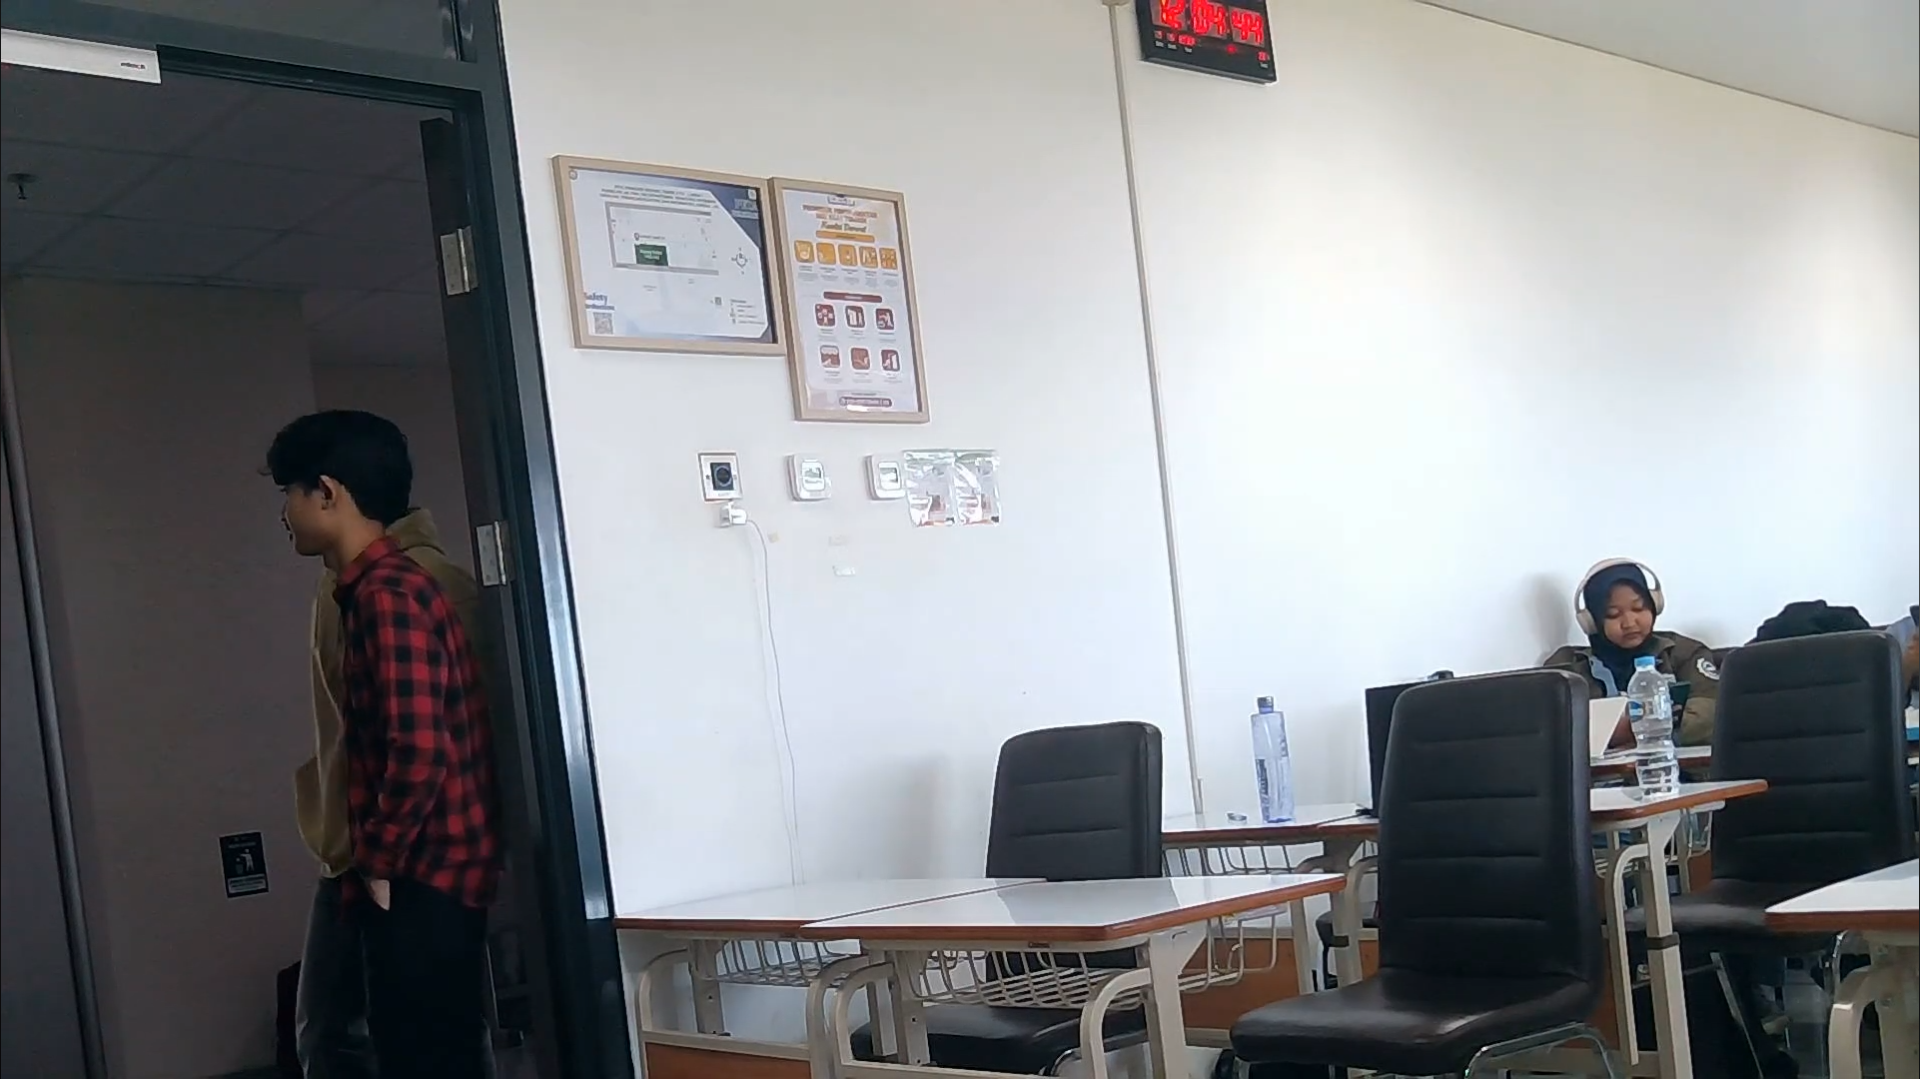
\includegraphics[width=0.9\textwidth]{gambar/Lampiran_video_1.png}
  \caption*{Cuplikan Uji Video Simulasi - Bagian 1}
\end{figure}

\begin{figure}[H]
  \centering
  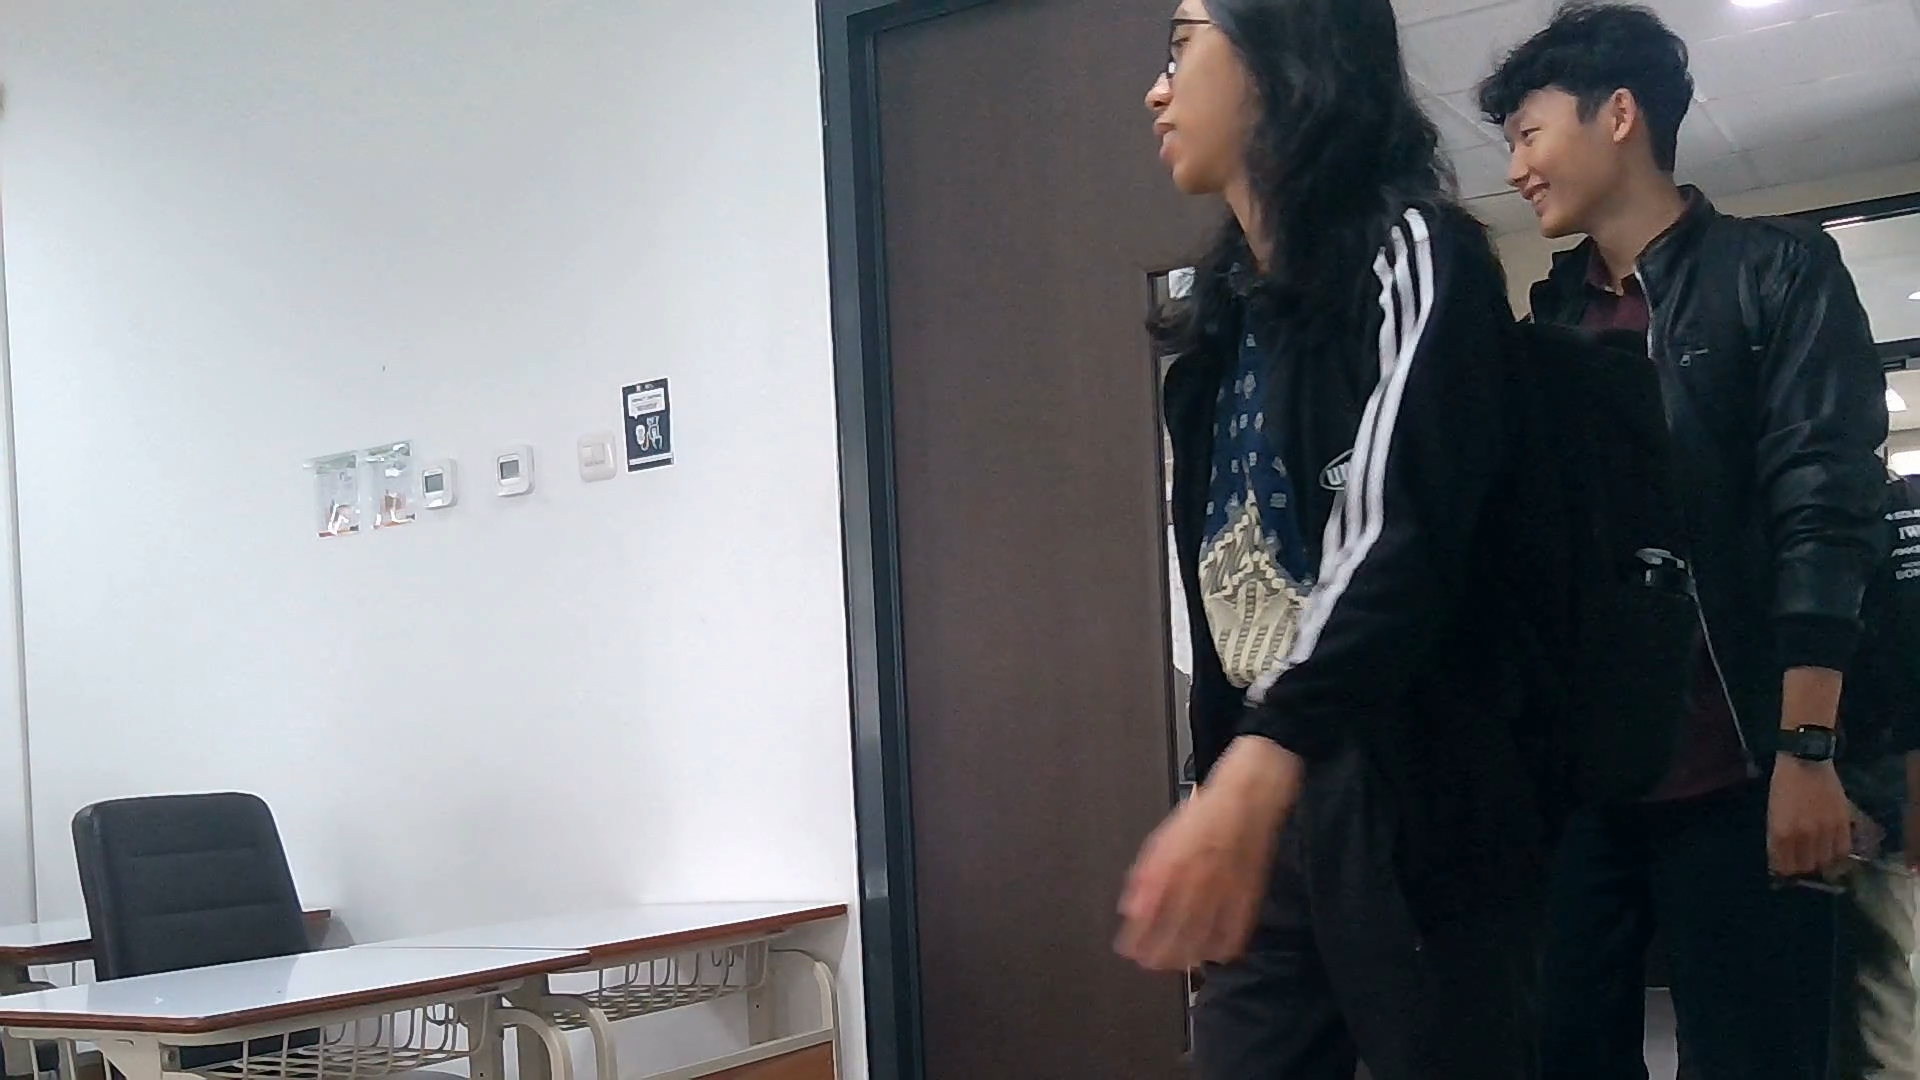
\includegraphics[width=0.9\textwidth]{gambar/Lampiran_video_2.png}
  \caption*{Cuplikan Uji Video Simulasi - Bagian 2}
\end{figure}
